\documentclass[11pt]{article}

\usepackage[a4paper]{geometry}
\geometry{left=2.0cm,right=2.0cm,top=2.5cm,bottom=2.5cm}

\usepackage{ctex} % 支持中文的LaTeX宏包
\usepackage{float} % 防止图片乱序
\usepackage{xeCJK} % 中文字体
\usepackage{amsmath,amsfonts,graphicx,subfigure,amssymb,bm,amsthm,mathrsfs,
            mathtools,breqn} % 数学公式和符号的宏包集合
\usepackage{algorithm,algorithmicx} % 算法和伪代码
\usepackage[noend]{algpseudocode} % 算法和伪代码
\usepackage{fancyhdr} % 自定义页眉页脚
\usepackage[framemethod=TikZ]{mdframed} % 创建带边框的框架
\usepackage{fontspec} % 字体设置
\usepackage{adjustbox} % 调整盒子大小
\usepackage{fontsize} % 设置字体大小
\usepackage{tikz,xcolor} % 绘制图形和使用颜色
\usepackage{multicol} % 多栏排版
\usepackage{multirow} % 表格中合并单元格
\usepackage{pdfpages} % 插入PDF文件
\usepackage{listings} % 在文档中插入源代码
\usepackage{lstautogobble} % 去掉源代码多余的空格
\usepackage{xcolor} % 支持彩色
\usepackage{caption} % 支持图片标题
\usepackage{wrapfig} % 文字绕排图片
\usepackage{bigstrut,multirow,rotating} % 支持在表格中使用特殊命令
\usepackage{booktabs} % 创建美观的表格
\usepackage{circuitikz} % 绘制电路图
\usepackage{zhnumber} % 中文序号(用于标题)
\usepackage{tabularx} % 表格折行
\usepackage{enumitem} % 枚举列表
\usetikzlibrary{circuits.ee.IEC} % 使用欧洲风格的电路符号
\usetikzlibrary{circuits.logic.US} % 使用美国风格的逻辑门
\usetikzlibrary{shapes.geometric, arrows.meta, positioning} % 使用流程图的库

% 设置字体
\definecolor{bluekeywords}{rgb}{0.13, 0.13, 1}
\definecolor{greencomments}{rgb}{0, 0.5, 0}
\definecolor{redstrings}{rgb}{0.9, 0, 0}
\definecolor{graynumbers}{rgb}{0.5, 0.5, 0.5}
\lstset{
    autogobble, % 自动移除代码前的空白(对齐代码块)
    columns=fixed, % 使得空格不可拉伸
    showspaces=false, % 不显示空格
    showtabs=false, % 不显示制表符
    breaklines=true, % 自动换行
    showstringspaces=false, % 在字符串中不特别显示空格
    breakatwhitespace=true, % 仅在空白处进行自动换行
    escapeinside={(*@}{@*)}, % 设置一个特殊的标记,允许在代码中插入LaTeX代码
    commentstyle=\color{greencomments}, % 注释的颜色设置为绿色
    keywordstyle=\color{bluekeywords}, % 关键字的颜色设置为蓝色
    stringstyle=\color{redstrings}, % 字符串的颜色设置为红色
    numberstyle=\color{graynumbers}, % 行号的颜色设置为灰色
    identifierstyle=\color{orange}, % 标识符颜色
    basicstyle=\small\ttfamily, % 基本字体样式:小号的等宽字体
    frame=single, % 单线边框
    framesep=12pt, % 边框与代码的间隔
    framerule=0.75pt, % 边框宽度
    xleftmargin=13pt, % 左边距
    xrightmargin=7pt, % 右边距
    tabsize=4, % 制表符宽度
    captionpos=t, % 标题位置在顶部
}
\DeclareCaptionFont{white}{\color{white}}
\DeclareCaptionFormat{listing}{\colorbox[cmyk]{0.43, 0.35, 0.35,0.01}
{\parbox{\textwidth}{\hspace{15pt}#1#2#3}}}
\captionsetup[lstlisting]{format=listing,labelfont=white,textfont=white,
                          singlelinecheck=false, margin=0pt,
                          font={bf,footnotesize}}

\usepackage{hyperref} % 目录,章节,超链接
\hypersetup{
    bookmarks=true,  % 生成书签
    bookmarksnumbered=true  % 书签带章节编号
}

% 轻松引用, 可以用\cref{}指令直接引用, 自动加前缀.
% 例: 图片label为fig:1
% \cref{fig:1} => Figure.1
% \ref{fig:1}  => 1
\usepackage[capitalize]{cleveref}
% \crefname{section}{Sec.}{Secs.}
\Crefname{section}{Section}{Sections}
\Crefname{table}{Table}{Tables}
\crefname{table}{Table.}{Tabs.}

\setCJKmainfont{Source Han Serif CN}
\setmonofont{JetBrains Mono NL}
\punctstyle{kaiming}
% 偏好的几个字体, 可以根据需要自行加入字体ttf文件并调用
% 注意要在自己系统安装字体, 以供调用

\renewcommand{\emph}[1]{\begin{kaishu}#1\end{kaishu}}

% 对 section 等环境的序号使用中文
\renewcommand \thesection{\zhnum{section}、}
\renewcommand \thesubsection{\arabic{subsection}}
\renewcommand \thesubsubsection{(\arabic{subsubsection})}

%%%%%%%%%%%%%%%%%%%%%%%%%%%
%改这里可以修改实验报告表头的信息
\newcommand{\name}{蓝宇舟}
\newcommand{\studentNum}{2022K8009918005}
\newcommand{\class}{B0911010Y-02}
%%%%%%%%%%%%%%%%%%%%%%%%%%%

\begin{document}

% 标题
\begin{center}
  \LARGE \bf 操作系统第四次作业
\end{center}

\begin{center}
  \emph{姓名} \underline{\makebox[7em][c]{\name}}
  % 如果名字比较长, 可以修改box的长度"8em"为其他值
  \emph{学号} \underline{\makebox[12em][c]{\studentNum}}
  \emph{班级} \underline{\makebox[15em][c]{\class}}\\
\end{center}


% 环境说明
\section{环境说明}

\begin{itemize}
    \item 操作系统:{\tt Arch Linux x86_64}
    \item 内核版本:{\tt Linux 6.10.7-zen1-1-zen}
    \item 编译器版本:{\tt gcc (GCC) 14.2.1 20240805}
\end{itemize}


% 作业
\section{作业}

\subsection{
    一个C程序可以编译成目标文件或可执行文件。目标文件和可执行文件通常包含{\tt text}、{\tt data}、{\tt bss}、{\tt rodata}段,程序执行时也会用到堆({\tt heap})和栈({\tt stack})
}

\subsubsection{
    请写一个C程序,使其包含{\tt data}段和{\tt bss}段,并在运行时包含堆的使用。请说明所写程序中哪些变量在{\tt data}段、{\tt bss}段和堆上
}

\noindent
我写的程序如下:

\lstinputlisting[language=C, caption={prog1.c}]{code/prog1.c}

\noindent
变量的位置如下:

\begin{tabular}{|c|c|c|}
    \hline
    变量 & 所在位置 & 原因 \\
    \hline
    {\tt a} & {\tt data}段 & 初始化的全局变量 \\
    \hline
    {\tt b} & {\tt bss}段 & 未初始化的全局变量 \\
    \hline
    {\tt c} & {\tt data}段 & 静态变量 \\
    \hline
    {\tt *p} & 堆上 & 通过{\tt malloc}函数分配得到 \\
    \hline
\end{tabular}

\subsubsection{
    请了解{\tt readelf}、{\tt objdump}命令的使用,用这些命令查看(1)中所写程序的{\tt data}和{\tt bss}段,截图展示
}

\noindent
如下图所示,可以看到{\tt data}段和{\tt bss}段的内容:

\begin{figure}[H]
    \centering
    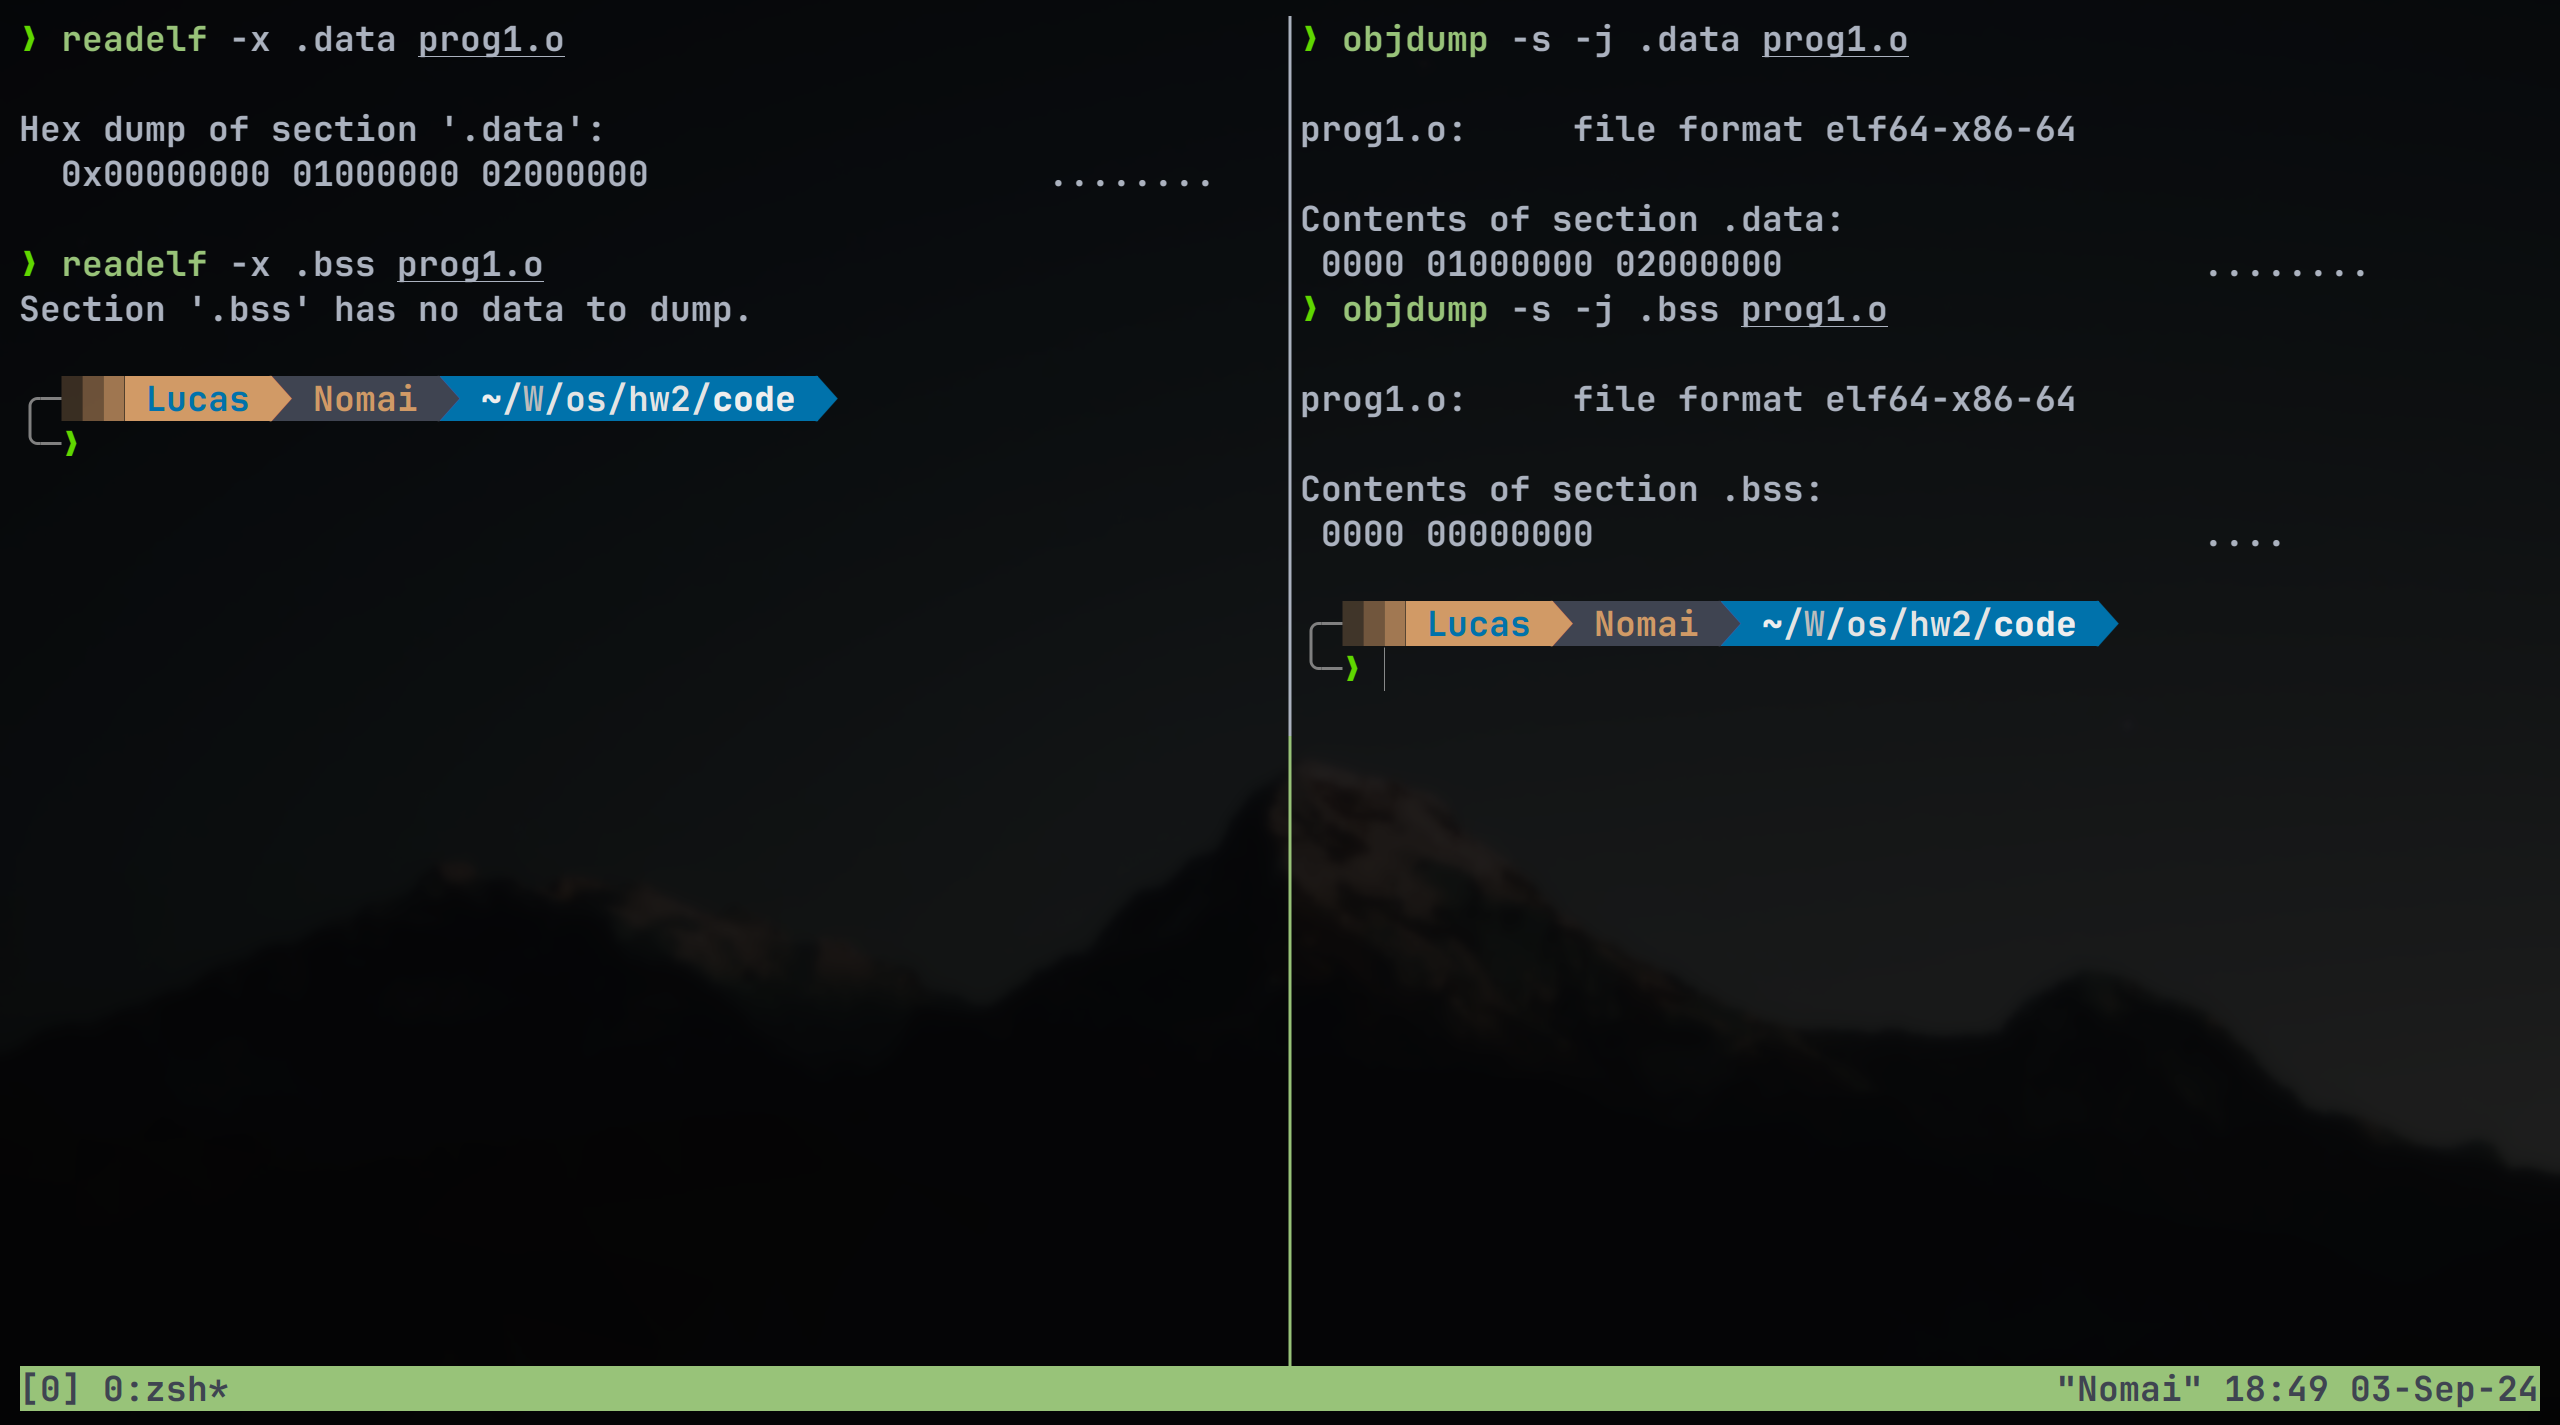
\includegraphics[width=1\textwidth]{fig/data_bss.png}
    \caption{{\tt data}和{\tt bss}段}
\end{figure}

\noindent
{\tt data}段的$0$和$1$刚好对应{\tt a}和{\tt c}的值,{\tt bss}段对应{\tt b}的值,符合预期。

\subsubsection{
    请说明(1)中所写程序是否用到了栈
}

\noindent
用到了栈,理由如下:

一方面,{\tt p}是一个局部变量,它的地址是在栈上分配的;另一方面,调用函数{\tt malloc()}的过程需要将返回地址压栈。

\subsection{
    {\tt fork}、{\tt exec}、{\tt wait}等是进程操作的常用API,请调研了解这些API的使用方法
}

\subsubsection{
    请写一个{\tt C}程序,该程序首先创建一个$1$到$10$的整数数组,然后创建一个子进程,并让子进程对前述数组所有元素求和,并打印求和结果。等子进程完成求和后,父进程打印{\tt "parentprocess finishes"},再退出
}

\noindent
我写的程序如下:

\lstinputlisting[language=C, caption={prog2.c}]{code/prog2.c}

\subsubsection{
    在(1)所写的程序基础上,当子进程完成数组求和后,让其执行{\tt ls -l}命令(注:该命令用于显示某个目录下文件和子目录的详细信息),显示你运行程序所用操作系统的某个目录详情。例如,让子进程执行{\tt ls -l /usr/bin}目录,显示{\tt /usr/bin}目录下的详情。父进程仍然需要等待子进程执行完后打印{\tt "parentprocess finishes"},再退出
}

\noindent
修改后的程序如下:

\lstinputlisting[language=C, caption={prog3.c}]{code/prog3.c}

\noindent
运行结果如下:

\begin{figure}[H]
    \centering
    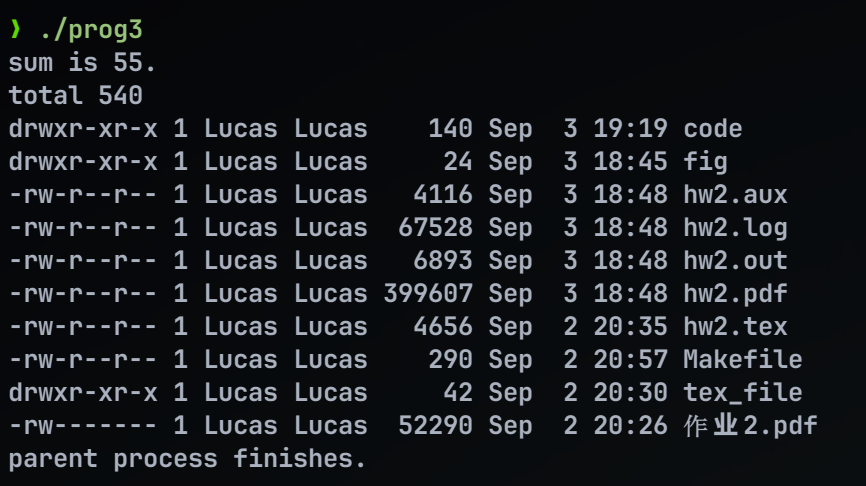
\includegraphics[width=1\textwidth]{fig/ls.png}
    \caption{运行结果}
\end{figure}

\subsubsection{
    请阅读XV6代码(https://pdos.csail.mit.edu/6.828/2024/xv6.html),找出XV6代码中对进程控制块({\tt PCB})的定义代码,说明其所在的文件,以及当{\tt fork}执行时,对{\tt PCB}做了哪些操作?
}

\noindent
{\tt PCB}的定义在{\tt kernel/proc.h}文件中,如下所示:

\begin{lstlisting}[language=C, caption={{\tt PCB}定义}]

    // Per-process state
    struct proc {
      struct spinlock lock;

      // p->lock must be held when using these:
      enum procstate state;        // Process state
      void *chan;                  // If non-zero, sleeping on chan
      int killed;                  // If non-zero, have been killed
      int xstate;                  // Exit status to be returned to parent's wait
      int pid;                     // Process ID

      // wait_lock must be held when using this:
      struct proc *parent;         // Parent process

      // these are private to the process, so p->lock need not be held.
      uint64 kstack;               // Virtual address of kernel stack
      uint64 sz;                   // Size of process memory (bytes)
      pagetable_t pagetable;       // User page table
      struct trapframe *trapframe; // data page for trampoline.S
      struct context context;      // swtch() here to run process
      struct file *ofile[NOFILE];  // Open files
      struct inode *cwd;           // Current directory
      char name[16];               // Process name (debugging)
    };

\end{lstlisting}

\noindent
当{\tt fork}执行时,对{\tt PCB}做了如下操作:

\begin{enumerate}
    \item 首先,定义变量{\tt p}和{\tt np},分别是指向父进程和子进程结构体的指针;
    \item 通过{\tt allocproc()}函数分配一个新的进程结构体,即子进程;
    \item 调用{\tt uvmcopy()}函数将父进程的内存信息复制给子进程;
    \item 将父进程的用户寄存器复制给子进程;
    \item 将子进程的返回值设置为{\tt 0};
    \item 用{\tt filedup()}函数将父进程的文件描述符复制给子进程;
    \item 用{\tt idup}函数将父进程的工作目录复制给子进程;
    \item 用{\tt safestrcpy()}复制进程名称;
    \item 释放子进程锁,设置子进程的父进程,设置子进程状态为可运行;
    \item 最后返回子进程的{\tt pid}。
\end{enumerate}

\subsection{
    请阅读以下程序代码,回答下列问题
}

\lstinputlisting[language=C, caption={程序代码}]{code/example.c}

\subsubsection{
    该程序一共会生成几个子进程?请你画出生成的进程之间的关系(即谁是父进程谁是子进程),并对进程关系进行适当说明
}

\noindent
该程序一共生成了$3$个子进程。进程关系如下:

\begin{figure}[H]
    \centering
    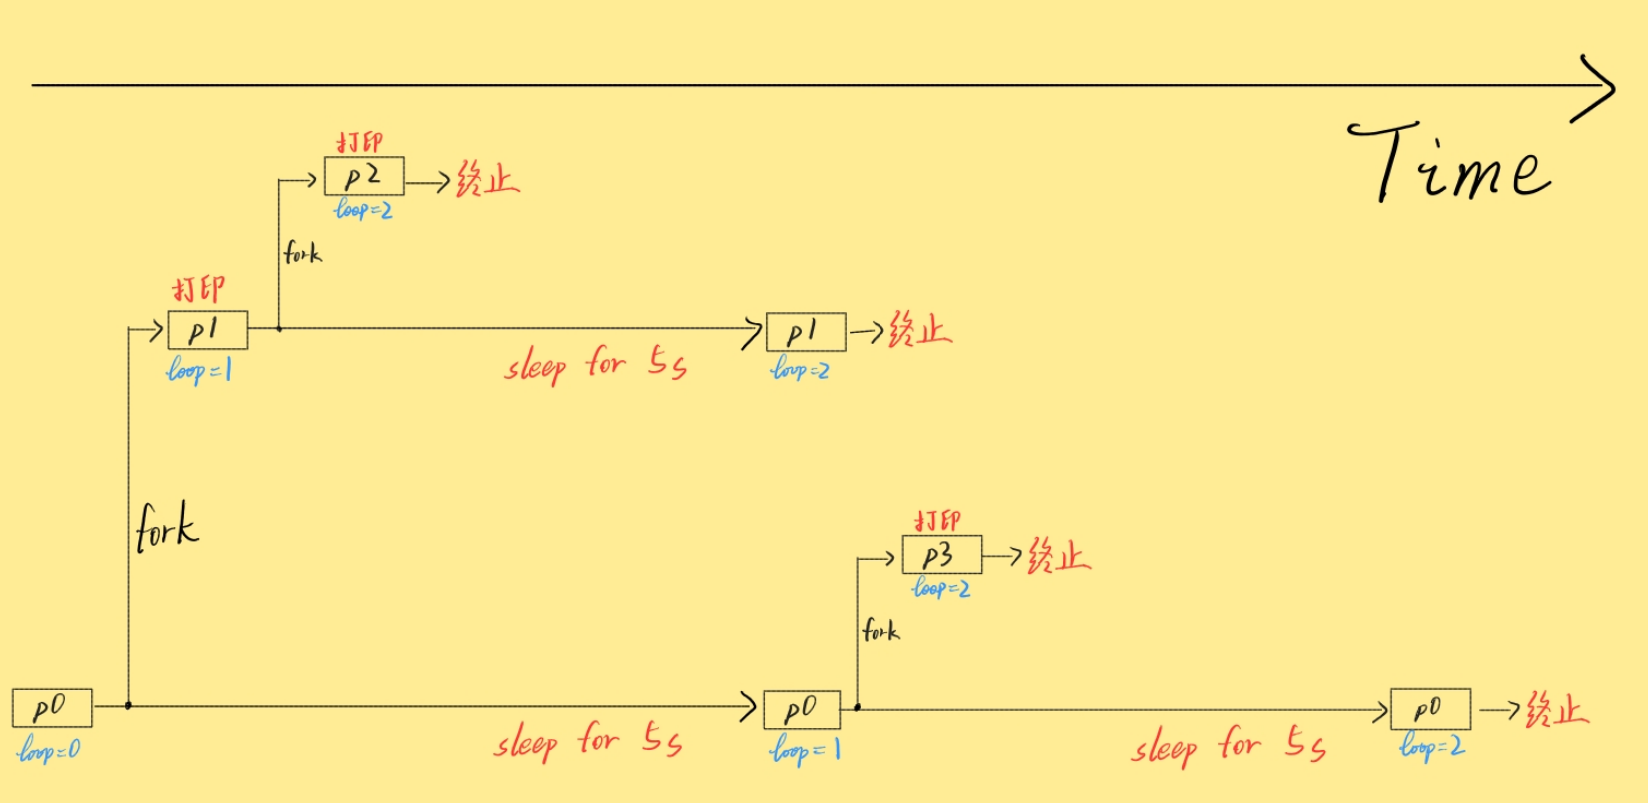
\includegraphics[width=1\textwidth]{fig/fork.png}
    \caption{进程关系}
\end{figure}

\noindent
说明:

\begin{enumerate}
    \item 设初始进程为{\tt p0},{\tt p0}在进行第一次{\tt fork()}系统调用后创造了子进程{\tt p1}。
    \item {\tt p0}休眠$5$秒;{\tt p1}在终端打印信息,{\tt loop}增加到$1$,同时立刻进行{\tt fork()}系统调用,创造子进程{\tt p2}。
    \item {\tt p2}在终端打印信息,{\tt loop}增加到$2$,结束循环,终止。
    \item {\tt p0}第一次休眠结束,{\tt loop}增加到$1$,进行{\tt fork()}系统调用后创建子进程{\tt p3},同时开始第二次休眠;{\tt p3}在终端打印信息后{\tt loop}增加到$2$,结束循环,终止。
    \item {\tt p1}休眠结束,{\tt loop}增加到$2$,结束循环,终止。
    \item {\tt p0}第二次休眠结束,{\tt loop}增加到$2$,结束循环,终止。
\end{enumerate}

\subsubsection{
    如果生成的子进程数量和宏定义{\tt LOOP}不符,在不改变{\tt for}循环的前提下,你能用少量代码修改,使该程序生成{\tt LOOP}个子进程么?
}

\noindent
有,我的方法是让父进程在创建完子进程后立刻终止,修改后代码如下:

\lstinputlisting[language=C, caption={程序代码}]{code/example_mod.c}


\end{document}
